\documentclass[10pt,a4paper]{article}
\usepackage[margin=16mm]{geometry}\usepackage{graphicx,booktabs,hyperref,xurl}
\begin{document}\title{E/P = 2, 2.5, 3: SiPM and ASIC clipping pilot}\author{NAUSICAA}\date{}\maketitle
The same 100 bb0nu source events, primary-pair checksums and drift distances are compared in both gases at E/P = 2, 2.5 and 3 kV/cm/bar. The user-specified EL variance ratios are J = 0.030, 0.015 and 0.025, respectively. The statistical SiPM uses 128 subdivisions per 250 ns bucket, PDE 0.3, gain 2.55e+06 and recovery time 73.4 ns. Electronics remain fixed at 0.5 PE RMS noise and a 1 mA upper current limit (611.9 PE per bucket). Full production remains stopped.
\begin{center}\resizebox{\textwidth}{!}{\begin{tabular}{llrrrrrrr}\toprule
Gas & E/P & J & Events & Charge retained \% & Photon cells clipped \% & Events with clipping \% & Before ASIC RMS \% & After ASIC RMS \% \\ \midrule
Pure Xe & 2 & 0.03 & 100 & 32.6 & 42.2 & 100 & 13.6 & 42.1 \\
Pure Xe & 2.5 & 0.015 & 100 & 27.3 & 49.1 & 100 & 16.0 & 43.4 \\
Pure Xe & 3 & 0.025 & 100 & 23.9 & 54.8 & 100 & 17.8 & 44.2 \\
Xe + 15\% He & 2 & 0.03 & 100 & 19.3 & 54.5 & 100 & 14.2 & 37.6 \\
Xe + 15\% He & 2.5 & 0.015 & 100 & 16.1 & 60.1 & 100 & 16.5 & 38.6 \\
Xe + 15\% He & 3 & 0.025 & 100 & 14.2 & 65.2 & 100 & 18.1 & 39.3 \\
\bottomrule\end{tabular}}\end{center}
Charge retained is the sum of ASIC output divided by the sum of SiPM input charge over the sample. The clipped-cell percentage uses only SiPM--bucket cells containing incident photons. The event percentage counts events with at least one clipped bucket. These three quantities have distinct denominators.

Event-total response spread is RMS/mean after subtracting the expected stationary dark baseline, correcting known attachment and dividing by deposited energy. SiPM recovery nonlinearity is retained in both columns. The before/after comparison measures the forward response spread under these corrections. All 100 events enter; the quoted widths are full-distribution RMS values. Each plotted ASIC distribution is divided by its own mean.
\clearpage\noindent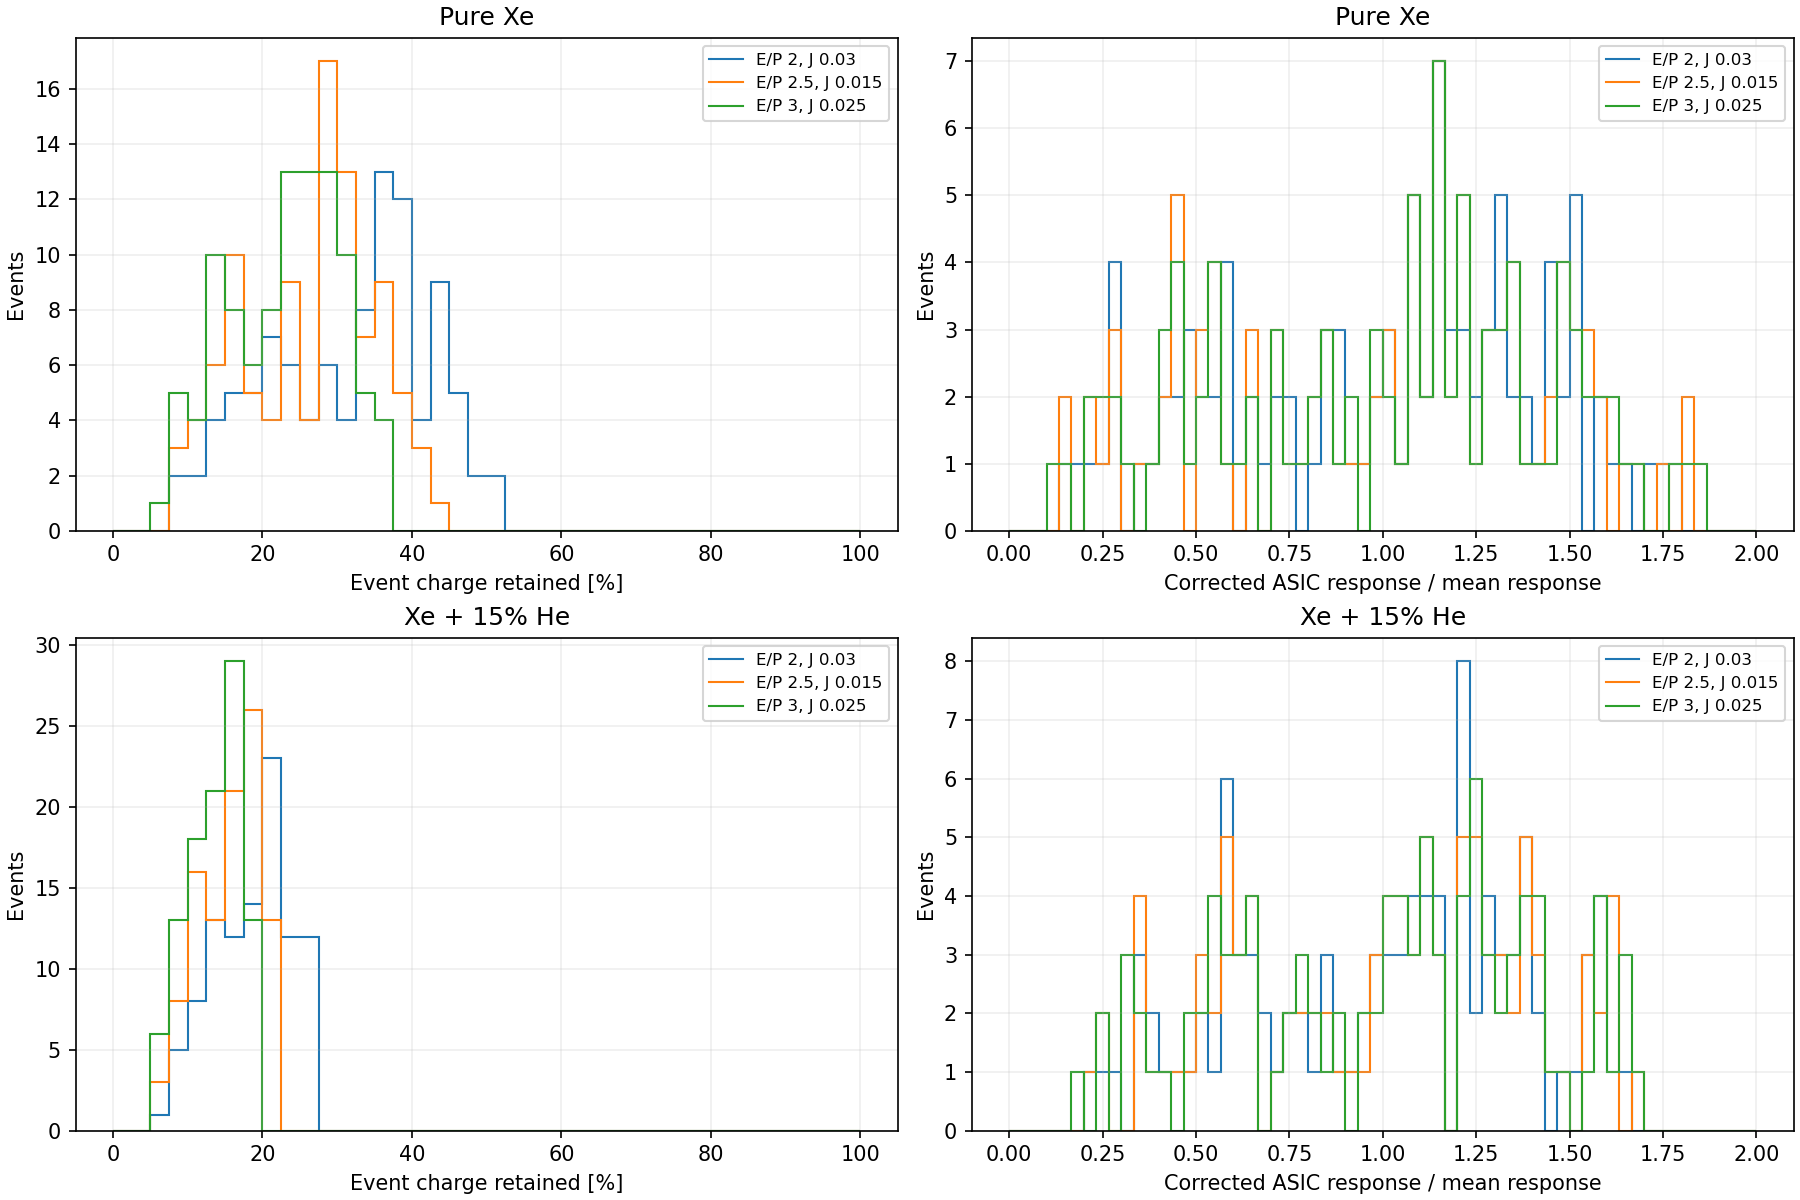
\includegraphics[width=\textwidth]{clipping_comparison.png}

Numerical results: \path{results/sipm_statistical_production_pilot/clipping_comparison.h5}.
The HTML counterpart links the complete response manifests for each operating point.
\end{document}
